\documentclass[a4paper,12pt]{article}
\usepackage{amsmath}
\usepackage{amssymb}
\usepackage{bigstrut}
\usepackage{fancyhdr}
\usepackage{graphicx}
\usepackage{subfigure}
\usepackage{pgfplots}
\usepackage{multirow}
\usepackage{caption}
\usepackage[a4paper, total={7in, 9in}]{geometry}
\pagestyle{fancy}
\fancyhead[le,ro]{\textbf{Sudip Kumar Kar(1911179)}}
%\pgfplotsset{compat=1.16}
\begin{document}
\title{Importance sampling in Monte Carlo Integration}
\author{Sudip Kumar Kar, 1911179}
\date{}
    \maketitle
    \section*{Theory}
    Monte Carlo Integration is a technique that uses probabilistic method to evaluate an integral. The principle of Monte Carlo integration relies on the Law of Large numbers, as a consequence there is no way to determine how many samples should be taken to give an accurate enough result, in addition, the standard deviation also goes as $1/\sqrt{N}$. The advantage of Monte Carlo integration is that it can be used to estimate an integral as long as one can sample from it, thus placing it in clear advantage for calculating multidimensional integrals where none of the standard techniques apply.\\
    Naively, one uses a uniform distribution to sample the values, but it may not always be wise to sample from a uniform distribution if certain values can contribute more towards an integral as compared to others, in such cases, computational time is wasted towards evaluation of quantities that may not contribute anything towards an integral. Thus, we choose the method of Importance sampling, where we use a distribution that closely resembles the variation in the original integrand, and then apply the Law of Large numbers to estimate the integral.\\
    Suppose, one wants to estimate the following integral,
    \begin{gather}
        \int_a^b f(x)dx \label{eqn:Mint}
    \end{gather}
    We divide and multiply the integrand by another distribution function $p(x)$ normalised over all possible values of x which in our case is $(-\infty,\infty)$,
    \begin{gather}
        \int_a^b \frac{f(x)}{p(x)}p(x) dx \stackrel{\text{Law of Large numbers}}{\longrightarrow} \frac{1}{N}\sum_{i=1}^N\frac{f(x_i)}{p(x_i)}=\mathcal{F}_N
    \end{gather}
    Where $\mathcal{F}_N$ is called the estimator. The variance in the calculation of the estimator is given as,
    \begin{gather}
        \sigma^2\left(\frac{f}{p}\right)=\frac{1}{N}\sum_{i=1}^N \left(\frac{f(x_i)}{p(x_i)}\right)^2-\left(\frac{1}{N}\sum_{i=1}^N\frac{f(x_i)}{p(x_i)}\right)^2
    \end{gather}
    From the expression above it is apparent that the closer $p(x)$ is to $f(x)$, the lesser the value of variance.\\
    Consider the case where $p(x)=\tilde{p}(x)/Z$ where $Z$ is the normalisation factor, in such a case, the integral becomes,
    \begin{gather}
        \int_a^b \frac{f(x)}{p(x)}p(x) dx =\int_a^b \frac{f(x)\tilde{p}(x)/Z}{\tilde{p}(x)/Z}\stackrel{\text{Law of Large numbers}}{\longrightarrow} \frac{Z}{N}\sum_{i=1}^N\frac{f(x_i)}{\tilde{p}(x_i)}=\mathcal{F}_N
    \end{gather}
    Thus, if $\tilde{p}(x)$ is not normalised, we must find $Z$ first to compute the value of the integral. Consequently, the variance also changes,
    \begin{gather}
        \sigma^2\left(\frac{f}{p}\right)=\frac{Z^2}{N}\sum_{i=1}^N \left(\frac{f(x_i)}{p(x_i)}\right)^2-\left(\frac{Z}{N}\sum_{i=1}^N\frac{f(x_i)}{p(x_i)}\right)^2
    \end{gather}
    Two problems have been considered to demonstrate the usefullness of Importance sampling.
    \section*{Problem 1}
    The following integral is to be evaluated,
    \begin{gather}
        \int_0^{10} e^{-2|x-5|} dx
    \end{gather}
    From figure. (\ref{fig:UvIsampp1}) it is apparent that sampling from the gaussian centered at $x=5$ will lead to much more accurate results.\\
    \begin{figure}[h!]
        \centering
        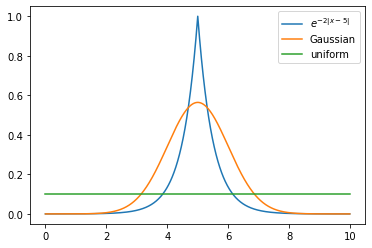
\includegraphics[width=0.5\linewidth]{p1_prob.png}
        \caption{\label{fig:UvIsampp1}Comparison between Uniform and Importance sampling}
    \end{figure}
    Unsurprisingly, when such a method is followed, the variance reduces significantly and the Estimate for the  integral stabilises quite early as it can be seen in figures (\ref{fig:UvIstdp1}-\ref{fig:UvIestp1}).
    \begin{figure}
        \centering
        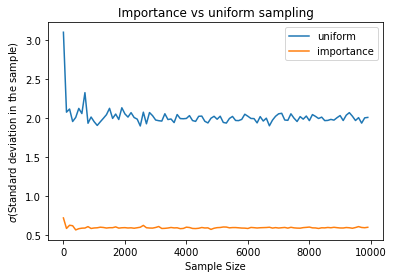
\includegraphics[width=0.5\linewidth]{p1_stdev.png}
        \caption{\label{fig:UvIstdp1}$\sigma$ Comparison between Uniform and Importance sampling}
    \end{figure}
    \begin{figure}
        \centering
        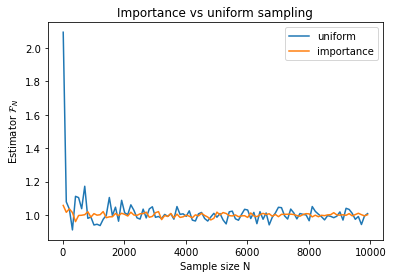
\includegraphics[width=0.5\linewidth]{p1_est.png}
        \caption{\label{fig:UvIestp1}Estimator Comparison between Uniform and Importance sampling}
    \end{figure}
    \newpage
    \section*{Problem 2}
    To demonstrate the versatility of the program in sampling from any kind of distribution, the following integral has been considered,
    \begin{gather}
        \int_{-\pi}^{\pi} \sin^2 x dx
    \end{gather}
    From figure (\ref{fig:UvIsampp2}), it is more apparent that the custom distribution $x^4e^{-0.8x^2}$ is a better distribution to sample from than an uniform one.\\
    \begin{figure}[h!]
        \centering
        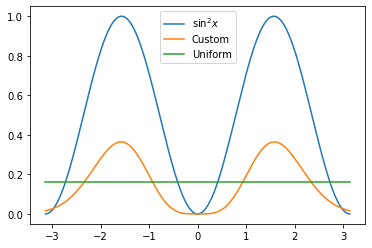
\includegraphics[width=0.5\linewidth]{p2_prob.png}
        \caption{\label{fig:UvIsampp2}Comparison between Uniform and Importance sampling}
    \end{figure}
    As expected in figures (\ref{fig:UvIstdp2}-\ref{fig:UvIestp2}), the results from Importance sampling yield a lower variance as compared to Uniform sampling in most cases, although it is true that a better choice of distribution can bring the results even closer to the true value.
    \begin{figure}
        \centering
        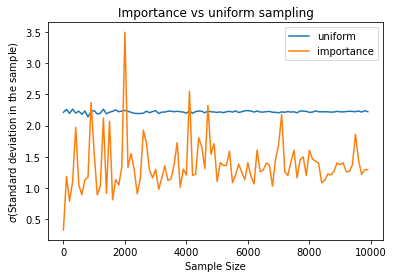
\includegraphics[width=0.5\linewidth]{p2_stdev.png}
        \caption{\label{fig:UvIstdp2}$\sigma$ Comparison between Uniform and Importance sampling}
    \end{figure}
    \begin{figure}
        \centering
        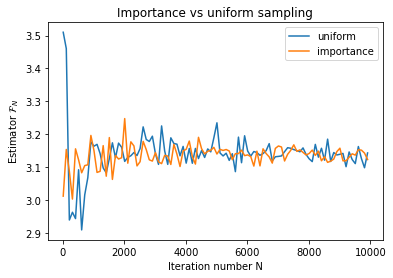
\includegraphics[width=0.5\linewidth]{p2_est.png}
        \caption{\label{fig:UvIestp2}Estimator Comparison between Uniform and Importance sampling}
    \end{figure}
    \newpage
    \section*{Conclusion}
    The theory and motivation behind Importance sampling in Monte Carlo integration was described and then two problems were used to demonstrate the effectiveness of Importance sampling, the results obtained confirmed the expectations from which it was established beyond any doubt that Importance sampling is crucial if one wants to minimise error in their calculations.
\end{document}